\documentclass[usletter, 11pt, titlepage]{article}
\title{Mapping Fractures using MicroCT Images}
\author{Omar Alamoudi}
\date{May 14, 2019}


\usepackage[margin = 1in]{geometry}
\setlength{\parskip}{0.25cm}
\renewcommand{\baselinestretch}{1.0}
\usepackage{mathtools, amssymb, subcaption, float}
\usepackage{grffile}
\usepackage{graphicx}
\graphicspath{{figures/}}


\usepackage{hyperref}
\def\chapterautorefname~#1\null{Chap.~(#1)\null}
\def\sectionautorefname~#1\null{Sec.~(#1)\null}
\def\subsectionautorefname~#1\null{Sec.~(#1)\null}
\def\figureautorefname~#1\null{Fig.~(#1)\null}
\def\tableautorefname~#1\null{Tab.~(#1)\null}
\def\equationautorefname~#1\null{Eq.~(#1)\null}

\newcommand{\Autoref}[1]{%
  \begingroup%
  \def\chapterautorefname~##1\null{Chapter~(##1)\null}%
  \def\sectionautorefname~##1\null{Section~(##1)\null}%
  \def\subsectionautorefname~##1\null{Sub--Section~(##1)\null}%
  \def\figureautorefname~##1\null{Figure~(##1)\null}%
  \def\tableautorefname~##1\null{Table~(##1)\null}%
  \def\equationautorefname~##1\null{Equation~(##1)\null}%
  \autoref{#1}%
  \endgroup%
}


\usepackage[style=authoryear]{biblatex}
\bibliography{references}


% a command to nubmer a particular line
\newcommand\numberthis{\addtocounter{equation}{1}\tag{\theequation}}


\begin{document}
\maketitle
\subsubsection*{A comment Nicola made during our meeting}
We should measure the point spread function, or edge spread function of our machine using properly calibrated materials (standard point, or cube, or bar) and use the resultant estimate of the point spread function in the image analysis. 


\section{Introduction}
In applications that are relevant to the utilization and understanding composite materials, particularly multi-phase materials, understanding the effective or apparent properties of such composites is essential for understanding how they behave under the influence of different physical and chemical processes. It is also very important to understand how constituents of such composites affect one another along the surfaces of contact. Rocks, soils, and rock melts are three complex composite material examples that geologist, geophysicists, and engineers encounter. Rocks are very rarely composed of a single physical material phase, in most likelihood, a rock sample is composed of at least two phases: a solid, and a fluid phase. The interaction between these phases is governed by the physical properties of each phase, and the law of conservation of mass, momentum, and energy of their system. With this broad view points in mind, a particular physical process that I am interested in is the processes governing fluid flow within fractured rocks, how the flow is affected by the introduction of fractures in such rocks, and the influence of varying the fluid pressure on these fractures, their capacity of storage and the flow of the fluids through them. 

Darcy's law shown in \autoref{eqn:Darcy's Law} \parencite{Darcy1856, Mavko2009} governs the conductivity of fluid within a cylindrical porous material sample with known geometry. The driving force of the fluid motion is the pressure gradient. Darcy's law does not make any explicit declarations about the spatial distribution, or shape of the pores within a rock specimen. On the other hand, the Kozeny--Carman \parencite{Carman1961, Mavko2009} describes the fluid flow through a cylindrical cavity in solid block see \autoref{eqn:Kozeny-Carman}. Imagine drilling a cylindrical cavity in the cylindrical sample with the known geometry with Radius R. \Autoref{eqn:Kozeny-Carman} describes the flow through that cavity. 

\begin{equation}
Q = - \frac{A}{L} \frac{\kappa }{\mu} \Delta p \label{eqn:Darcy's Law}
\end{equation}

\begin{equation}
Q = - \frac{1}{L} \frac{\pi R^4}{8\mu} \Delta p \label{eqn:Kozeny-Carman}
\end{equation}

\begin{equation}
\kappa = \frac{\pi R^4}{8A} \label{eqn:perm}
\end{equation}
Comparing \autoref{eqn:Darcy's Law} and \autoref{eqn:Kozeny-Carman}, \autoref{eqn:perm} shows that there a dependence of permeability on the cross sectional area of the sample, and the radius of the cavity. Considering an alternative case where we have fractures, one can deduce that we can estimate or predict the relationship between a rock sample geometry and fractures within the sample that would be the primary conduit of fluid flow. Therefore, the use of microCT images to map fractures is an important first step to understanding such relationship. 

Considering a single two-dimensional slice from a three-dimensional microCT volume data of two half-cylinder of a rock sample, \cite{Ketcham2010} have demonstrated the applicability of what the authors call the Inverse Point Spread Function method (IPSF) in measuring the apparent and true aperture of fractures from microCT volumes. Using this method requires visually inspecting and detecting the fractures in the image, then measuring them. An alternative approach proposed by \cite{Voorn2013} employs computing the Hessian to detect multi-scale fractures within a sample. In the paper, we discuss the application of \cite{Voorn2013} approach on synthetic images as a first step in attempting to detect fractures with the aim to eventually measure them. 

\section{Methods}
Our main objective is to improve the ability to detect, and henceforth measure fractures in microCT images acquired of rock samples. The approach followed is a similar to, if not the same as, the one described in \cite{Voorn2013}. To demonstrate this approach in detecting fractures, computed the Hessian of the synthetic images, and finally conducted analysis to map the fracture features from the images. The description of these steps follows in the same order stated above. 

\subsection{Synthetic Image Generation} \label{sec:Synthetic Fractures}
The workflow used in generating the synthetic fracture images was done using MATLAB. A user specified array of fracture apertures specified as an integer of pixels/voxels, i.e. [1,2,3,4,6] as shown in \autoref{fig:Synthetic images}, an integer number of pixels/voxels representing the length and width of the desired image, and an estimate of the signal to noise ratio (SNR) are used as input arguments. An equally spaced fractures are drawn in an image as pixels with the gray value zero in a background with gray value one. Four different images are generated in two sets. The first set is of two "sharp" images, and the other two are blurred by convolving the sharp image with a 3-by-3 (-by-3 in 3D) box filter. The blurred images are an attempt to represent the effect of the Point Spread Function (PSF) of a microCT machine \parencite{Ketcham2010}. Random noise was added to one of each set to observe and quantify the effect of random noise. The result of this workflow is a two-dimensional image with the specified fractures apertures as the apparent fractures, but since our objective is to map fractures, a plate like geometrical features, \cite{Voorn2013} have stated that two-dimensional images are insufficient in mapping fractures.  To generate a three-dimensional image with fractures that are vertically oriented, a stack of three of same image are superimposed on one another. For the images that contain noise, three different realizations of noise are stacked to preserve the randomness of noise. \Autoref{fig:Synthetic images} shows the middle slice of a three-dimensional image with input parameters [1,2,3,4,6] for fracture apertures, 100 voxels for the length of the image, and 10 for the SNR. 

\begin{figure}[!h]
\centering
    \begin{subfigure}[b]{0.5\textwidth}            
            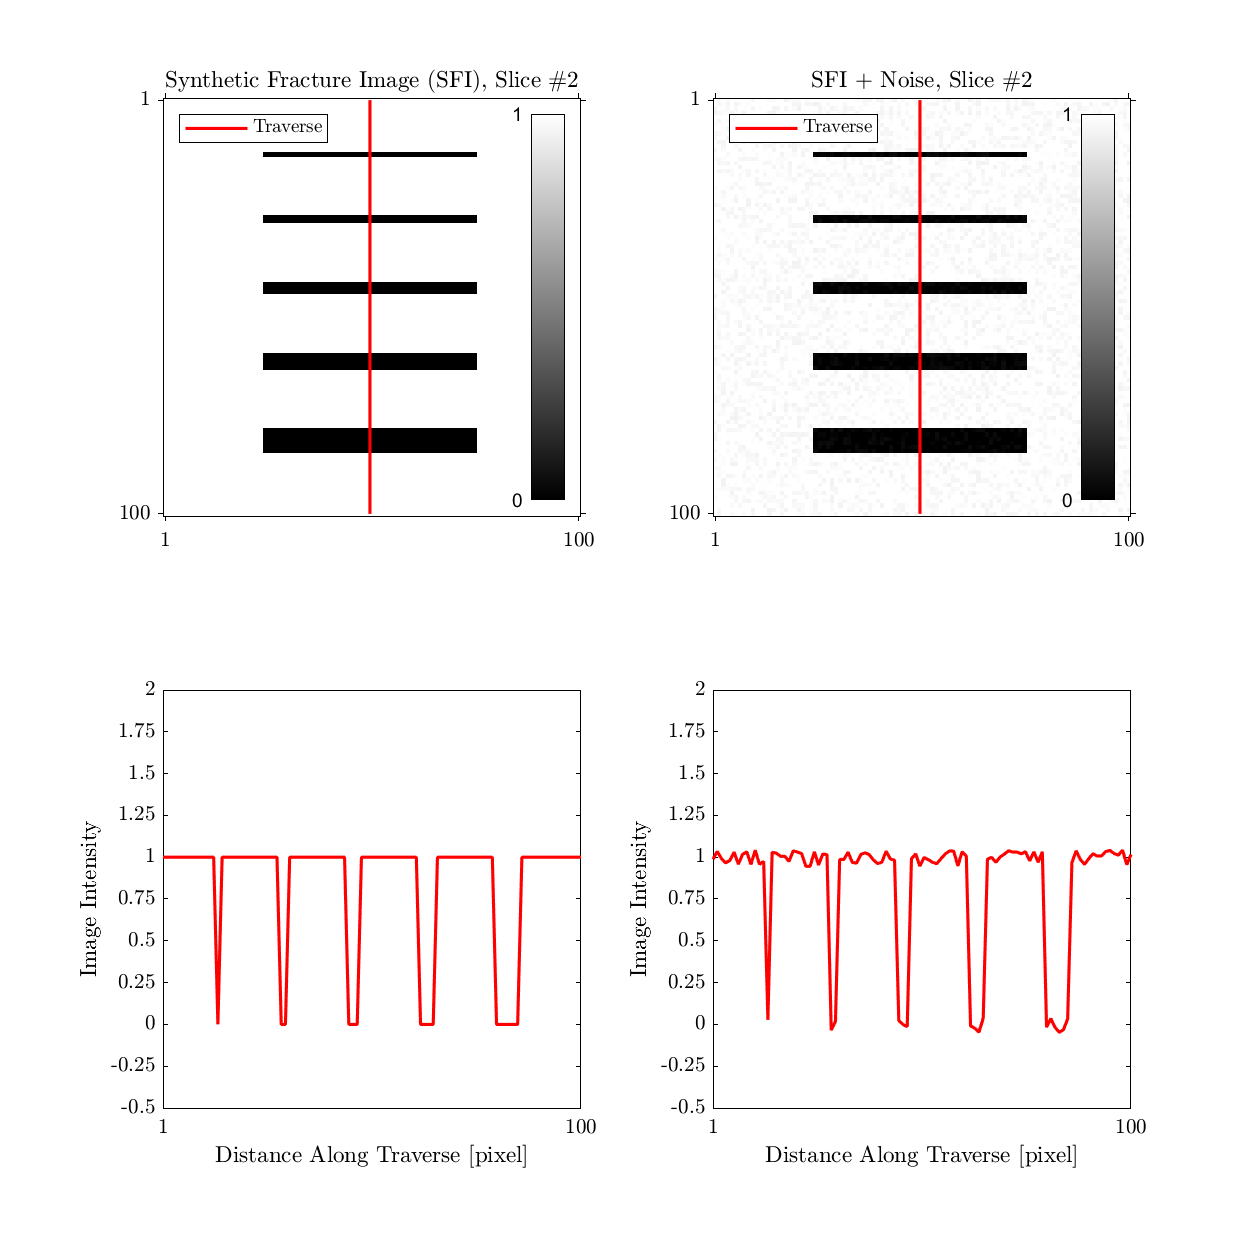
\includegraphics[width=\textwidth]{3DSyntheticFractureImages.png}
            \caption{Set of "sharp" images}
            \label{fig:Sharp images}
    \end{subfigure}%
     %add desired spacing between images, e. g. ~, \quad, \qquad etc.
      %(or a blank line to force the subfigure onto a new line)
    \begin{subfigure}[b]{0.5\textwidth}
            \centering
            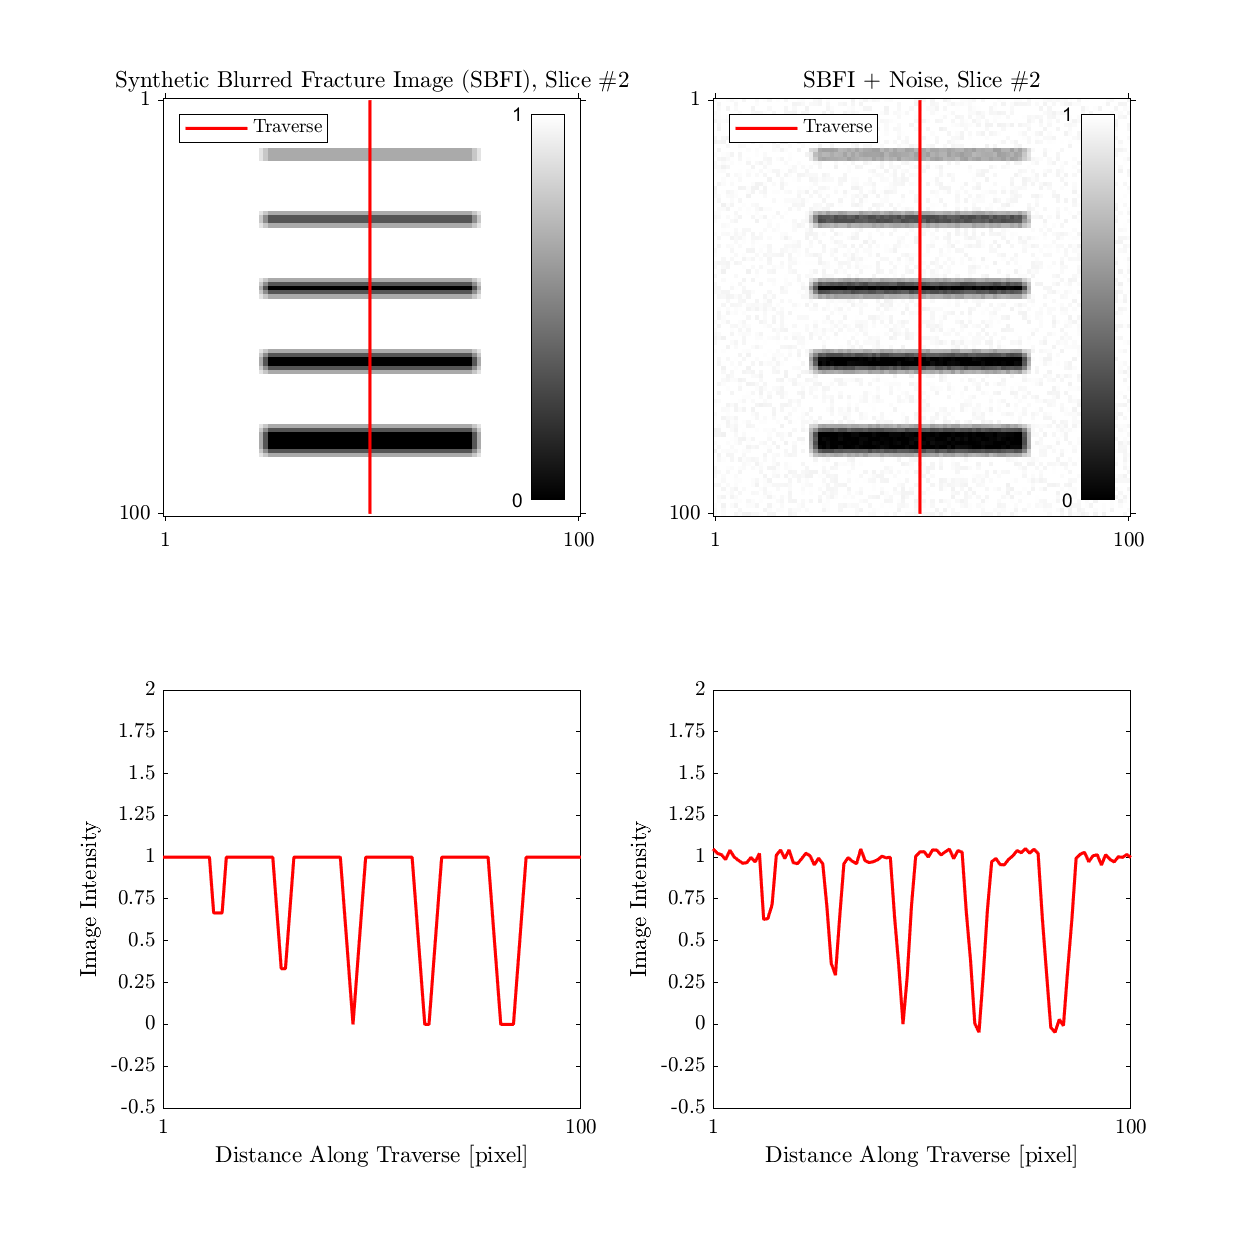
\includegraphics[width=\textwidth]{3DSyntheticBlurredFractureImages.png}
            \caption{Set of blurry images}
            \label{fig:Blurry images}
    \end{subfigure}
    \caption{The middle slice of a three-dimensional synthetic images. Top row shows the images, and the bottom row shows a traverse along the vertical red line. }
    \label{fig:Synthetic images}
\end{figure}

\subsection{Computing the Hessian} \label{sec:The Hessian}


To compute the Hessian of a microCT image, consider a three dimensional Euclidean domain $E^3$ representing the domain of a microCT image, and given a scalar valued field $\phi: E^3 \rightarrow \mathbb{R}$ representing the gray value of every voxel. The Hessian of the scalar field $\phi$ is $\mathbf{H}(\phi)$ as shown in \Autoref{eqn:hessian}. 

\begin{align*}
\mathbf{H} & = 
\begin{bmatrix}
I_{xx} & I_{xy} & I_{xz} \\
I_{yx} & I_{yy} & I_{yz} \\
I_{zx} & I_{zy} & I_{zz}
\end{bmatrix} \numberthis \label{eqn:hessian}
\intertext{Where} 
I & = \text{microCT image gray value field or image intensity} \\
I_{ij} & = \frac{\partial}{\partial i } \frac{\partial }{\partial j} I. \qquad i,j = [x,y,z] \numberthis \label{eqn:Second Derivative of I}
\end{align*}

The Hessian is a tensor value function $\mathbf{H}: E^3 \rightarrow \mathbb{R}^3 \times \mathbb{R}^3$. It has nine components six of which are unique, as the Hessian is symmetric. Organizing the Hessian componenets in a 3-by-3 matrix, $H_{ij}$ denotes the component of the ith row and jth column where $i,j = [x,y,z]$. Here $x, y$, and $z$ are orthogonal coordinates of our Euclidean space $E^3$. Since microCT images, or digital images in general, are discrete in nature, the computation of the derivatives can be done by finite differences. But that is not adequate. A \emph{multi-scale} technique is rather used. An over view of such technique is provided by \cite{Lindeberg1998}. This technique considers different scales of particularly edge features, in our case represented by fractures. For example, the second derivative $I_{xy} = \frac{\partial }{\partial x} (\frac{\partial I}{\partial y})$ of a three-dimensional image represented by $I = I(x,y,z)$ is computed as following:
\begin{align*}
I_{xy} & = \alpha \left[I * G_{xy}(x,y,z,s) \right] \numberthis \label{eqn:I xy}
\intertext{Where}
\alpha & = \text{Normalization factor} \\
G(x,y,z,s) & = \beta \exp\left\{ -\frac{1}{2s^2} \left[ \left(x - x_0\right)^2 + \left(y - y_0 \right)^2 + \left(z-z_0 \right)^2 \right] \right\} \quad (\text{Gaussian})\\
\beta & = \text{Amplitude of the Gaussian, normalization factor}
\end{align*}

\begin{figure}[!h]
\centering
    \begin{subfigure}[b]{0.5\textwidth}            
            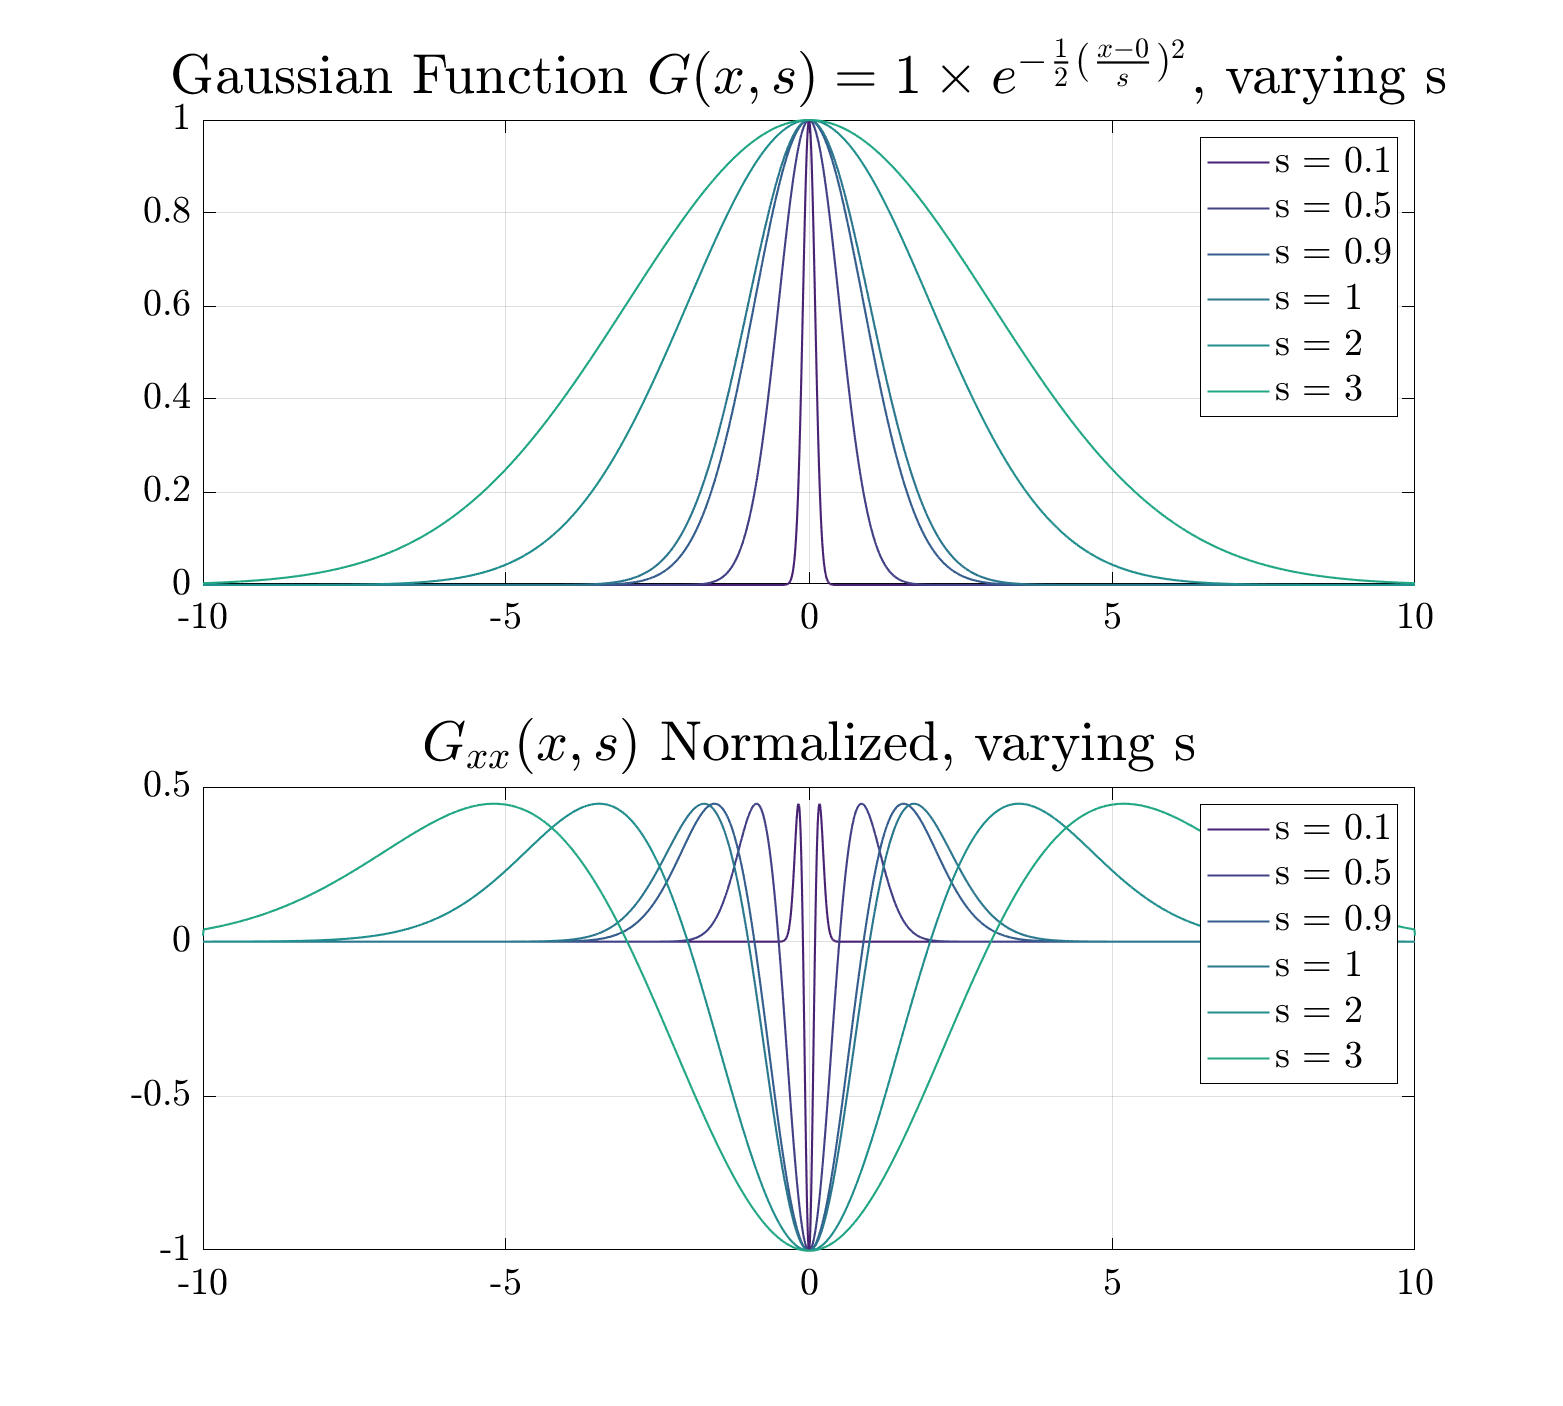
\includegraphics[width=\textwidth]{gaussian_continuous.png}
            \caption{Continuous}
            \label{fig:Gaussian cont}
    \end{subfigure}%
     %add desired spacing between images, e. g. ~, \quad, \qquad etc.
      %(or a blank line to force the subfigure onto a new line)
    \begin{subfigure}[b]{0.5\textwidth}
            \centering
            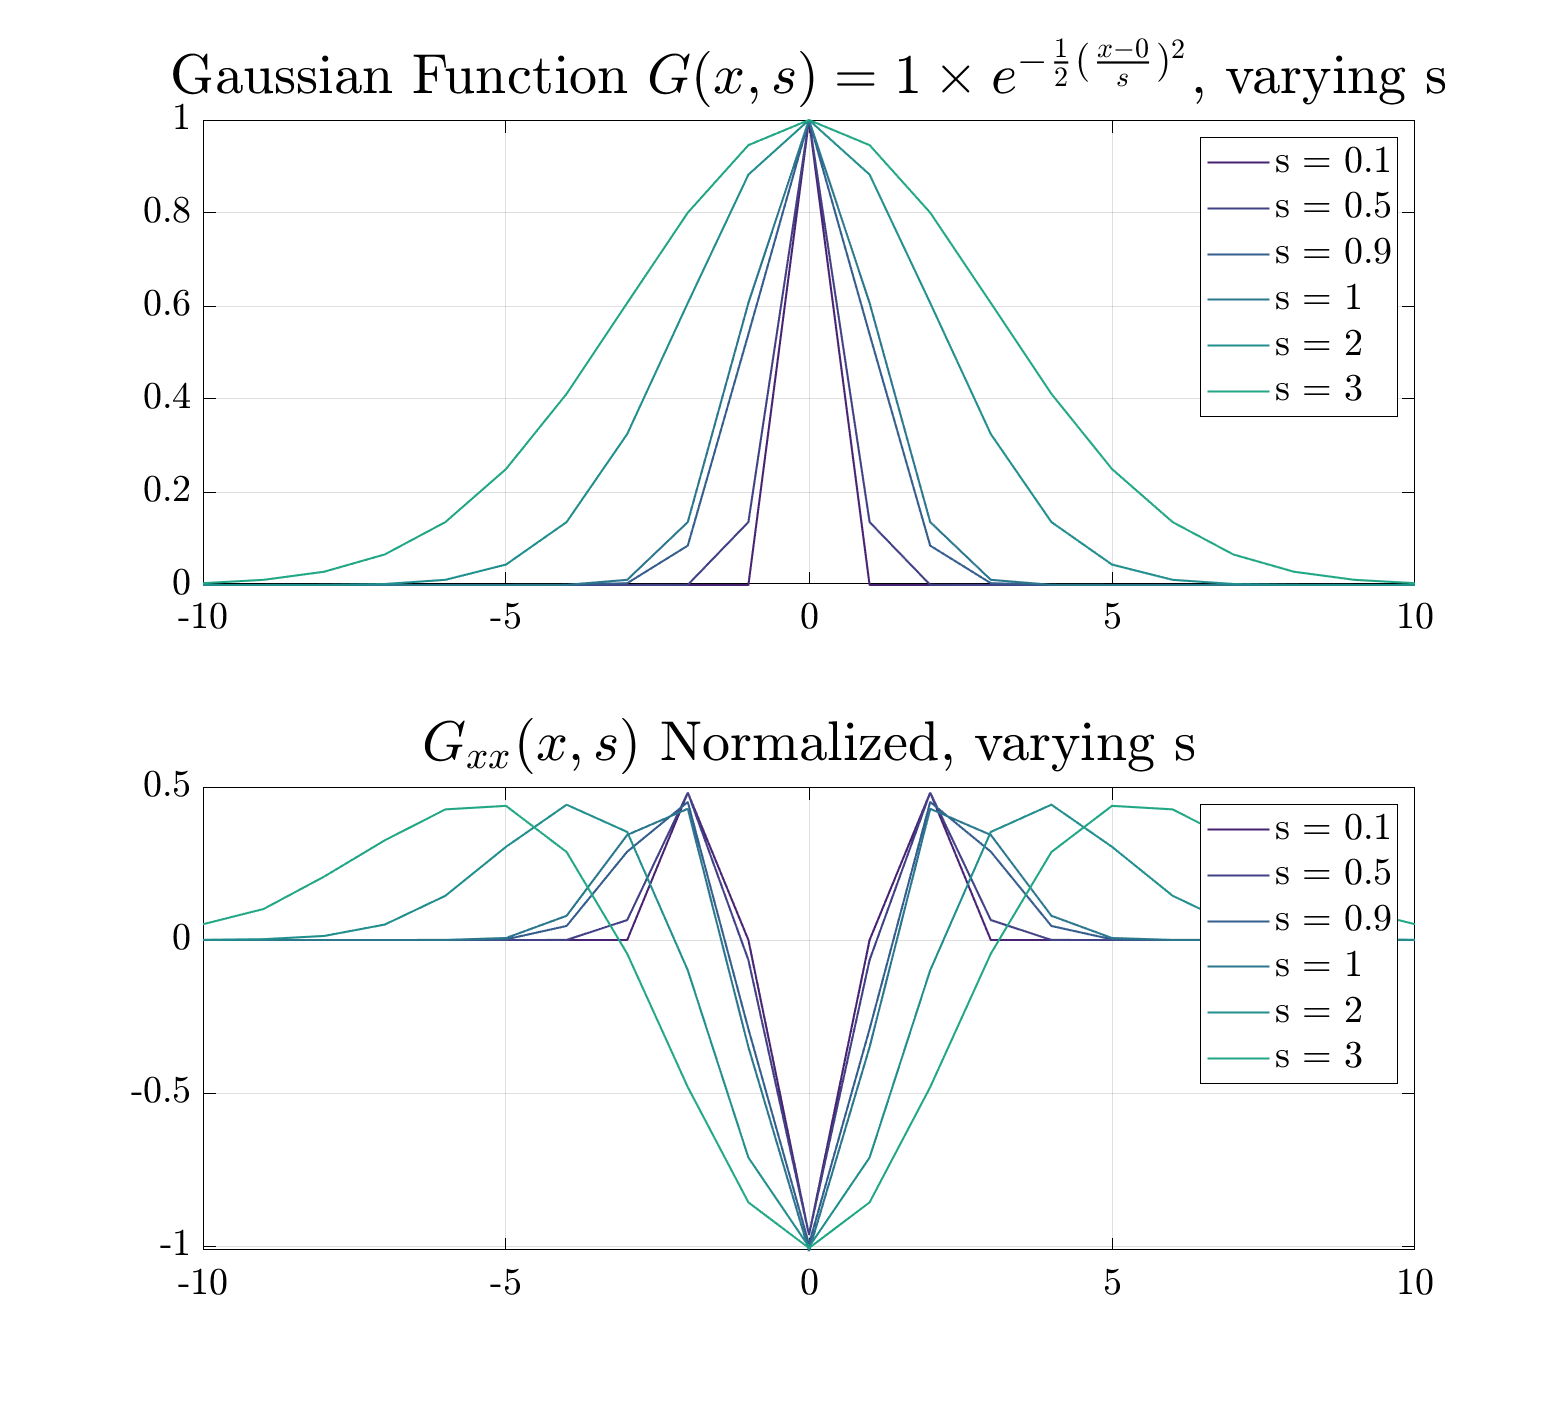
\includegraphics[width=\textwidth]{gaussian_discrete.png}
            \caption{Discrete}
            \label{fig:Gaussian disc}
    \end{subfigure}
    \caption{One-dimensional Gaussian function and  $G_xx(x,s)$ with varying $s$ in continuous and discrete forms.}
    \label{fig:Gaussian function}
\end{figure}

\Autoref{fig:Gaussian function} shows a one-dimensional Gaussian function and the second derivative with respect to $x$ in a continuous and a discrete form. The second derivative is equivalent to the $G_{xx}$ component that is convolved with the intensity of the image as shown in \autoref{eqn:I xy}. It is important to note that all of the operations carried out here is done using the discrete form. Different curves in \autoref{fig:Gaussian function} correspond to a different scaling parameter $s$. Darker colors correspond to small $s$, while brighter colors correspond to a larger $s$. 

For every single synthetic image of the set generated, we computed the all nine components of the Hessian for each voxel for different values of the scaling parameter $s$. This was done by first choosing a value of $s$, then generating a three-dimensional Gaussian filter, $G(x,y,)$, using the MATLAB function \texttt{fspecial3} with a \emph{filter size of 19}, computing the nine derivatives, $G_{ji}(x,y,x)$ for $i,j = [x,y,z]$, that are used in \autoref{eqn:I xy}, then convolving the result with the images while choosing $\alpha$ such that   Looking at the bottom plot of \autoref{fig:Gaussian cont}, each curve can be defined by it largest trough bounded by two smaller peaks. The distance that defines the largest trough for every curve between the two points (closest to zero) intersection the horizontal axis is $2s$. 

\subsection{Fracture Mapping Analysis}
After computing the all nine components of the Hessian for every voxel of the synthetic images for every value of $s$, we compute the eigenvalues $\lambda_1,~ \lambda_2,~\lambda_3$, where $\lambda_1 < \lambda_2 < \lambda_3$. For every value of $s$, for plate like features, we expect one of the eigenvalues to have a large magnitude while the other two to have small magnitudes. Using the same criteria proposed by \cite{Voorn2013}, we can then define a new value $A_s$ for every voxel such that 
$$A_s = \begin{cases}
\lambda_3 - |\lambda_2| - |\lambda_1| &\quad \text{if} ~ (\lambda_3 - |\lambda_2| - |\lambda_1|) > 0\\
0 \qquad &\text{otherwise}
\end{cases} $$
where $s$ here stands for the scaling parameter. We then normalize $A_s$ such that $B_s = \frac{A_s}{\max(A_s)}$, and finally define another quantity $C_s$ such that 
$$
C_s = \begin{cases}
1 & \text{if} ~ B_s > 1 - \gamma \\
0 & \text{otherwise}
\end{cases}
$$
$\gamma$ is an arbitrary tolerance that I chose to be $0.40$ in my application. I then summed up all of $C_s$ for all scaling parameters used. In my case, since this analysis was applied to a synthetic image set, the scaling parameter was set to be $s = \frac{1}{2}  [1,2,3,4,6]$. \Autoref{fig:Fracture Mapping Analysis} shows the results of conducting the above steps for every value $s$. 

The final step is normalizing the final cumulative result shown in \autoref{fig:Fracture Mapping Analysis}, and inverting the image to match the original synthetic image as shown in \autoref{fig:Results}. 

\begin{figure}[!h]
\centering
\includegraphics[width = \textwidth]{"SFI,s = 0.5, Aperture = 1, Frac (1 of 5), hsize = 19"}
\includegraphics[width = \textwidth]{"SFI,s = 1, Aperture = 2, Frac (2 of 5), hsize = 18"}
\includegraphics[width = \textwidth]{"SFI,s = 1.5, Aperture = 3, Frac (3 of 5), hsize = 19"}
\includegraphics[width = \textwidth]{"SFI,s = 2, Aperture = 4, Frac (4 of 5), hsize = 18"}
\includegraphics[width = \textwidth]{"SFI,s = 3, Aperture = 6, Frac (5 of 5), hsize = 18"}
\caption{From top to bottom, incremental results for every scaling value $s$. Left to right of each row $A_s$, $B_s$, $C_s$, and the cumulative addition of the current step and all of the previous ones of $C_s$. Note here that the bottom row shows the final result of the analysis before normalizing and inverting the image. }
\label{fig:Fracture Mapping Analysis}
\end{figure}

\section{Results and Discussion}
\Autoref{fig:Results} shows the result of my analysis on all four synthetic images.  We can see from the traverse profiles that we are able to detect the fractures of different scales in the sharp images, but we are unable to detect the smallest fracture in the blurred images. We can also see that the effect of random noise with SNR = 10 on the final result is minimal. Although we are able to detect the fractures, the fracture apertures do not visually match the corresponding fractures in the original synthetic image. 

\begin{figure}[!h]
\centering
    \begin{subfigure}[b]{0.5\textwidth}            
            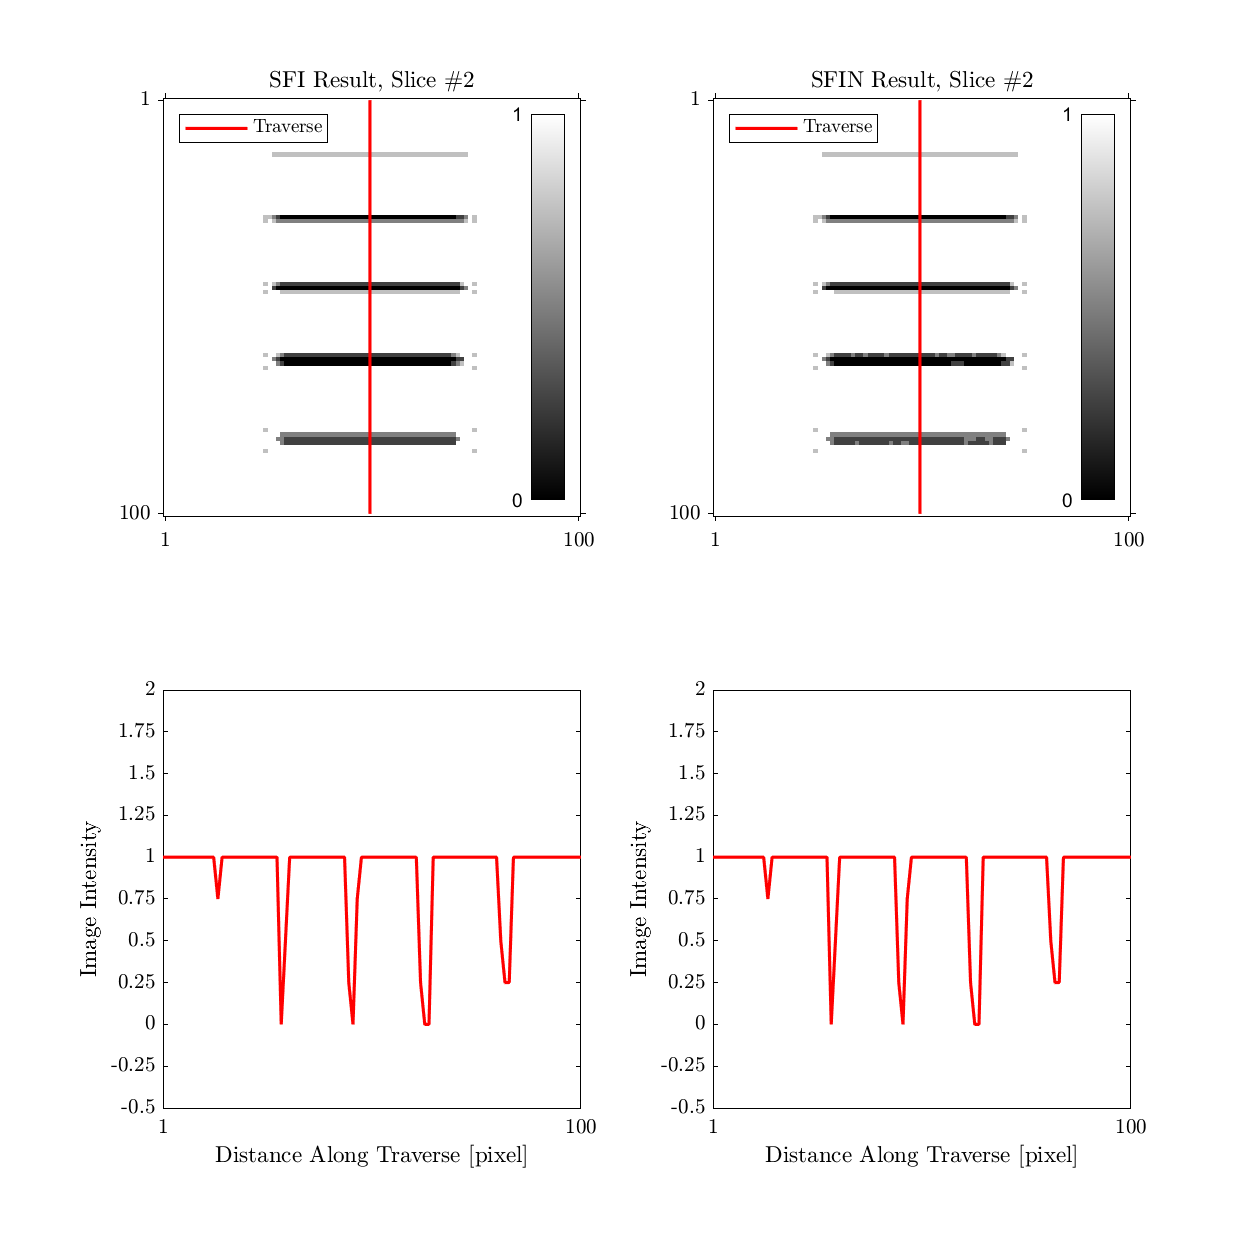
\includegraphics[width=\textwidth]{HessianResultsSFI_N}
            \caption{Result set of "sharp" images}
            \label{fig:Sharp images result}
    \end{subfigure}%
     %add desired spacing between images, e. g. ~, \quad, \qquad etc.
      %(or a blank line to force the subfigure onto a new line)
    \begin{subfigure}[b]{0.5\textwidth}
            \centering
            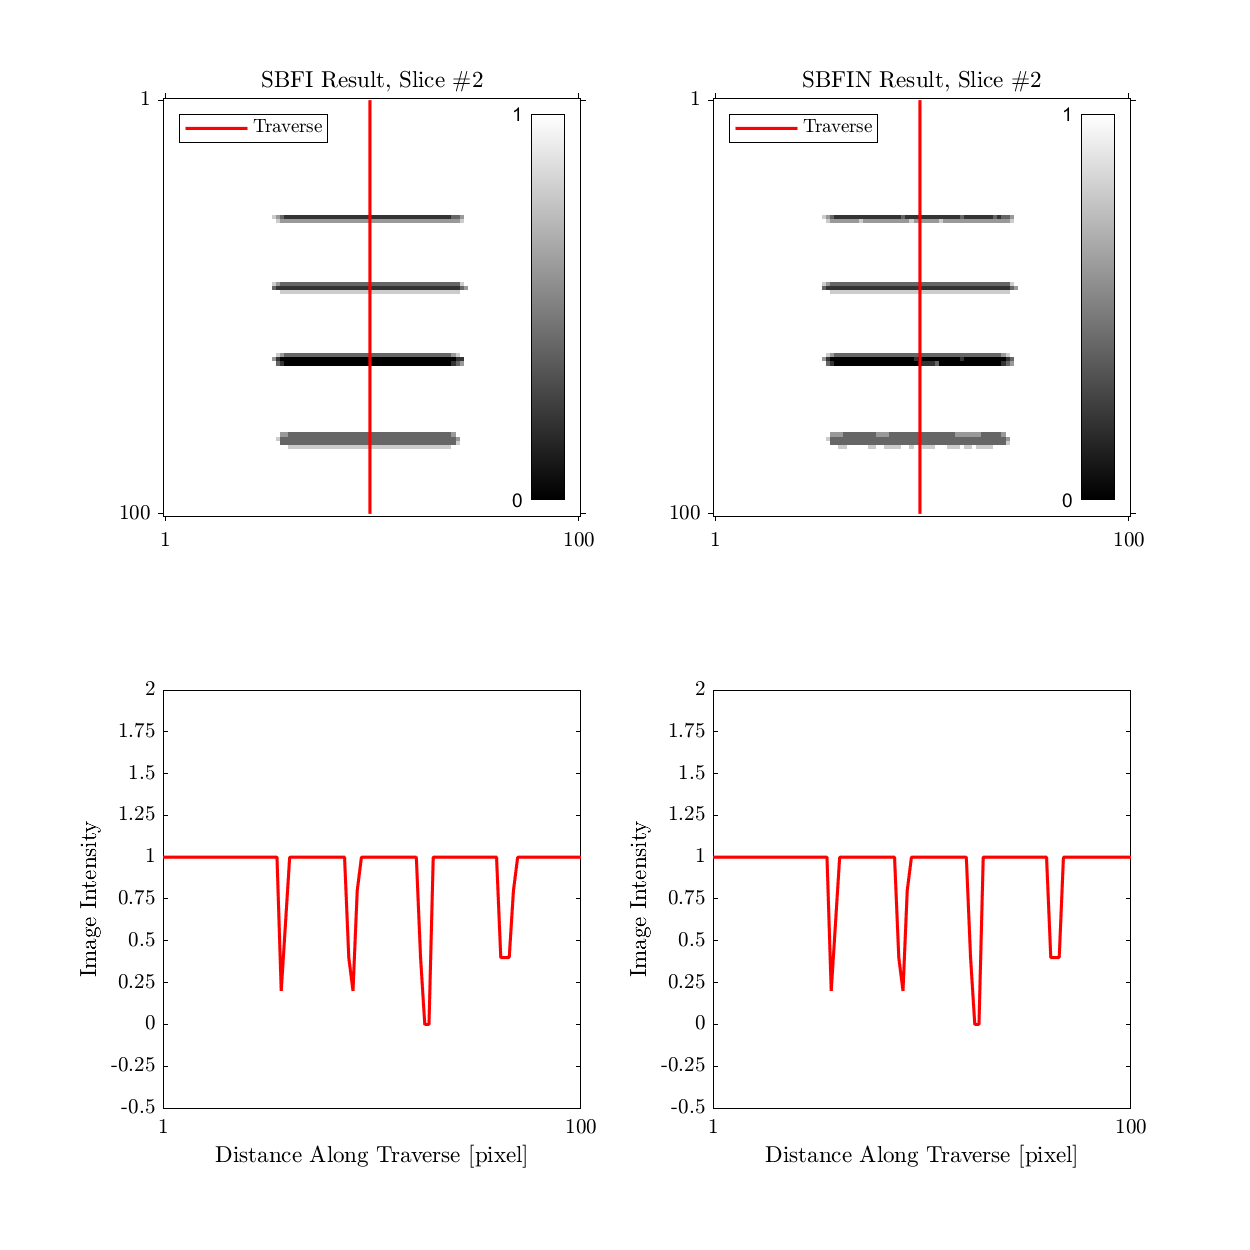
\includegraphics[width=\textwidth]{HessianResultsSBFI_N.png}
            \caption{Result set of blurry images}
            \label{fig:Blurry images result}
    \end{subfigure}
    \caption{The middle slice of a three-dimensional resultant images. Top row shows the images, and the bottom row shows a traverse along the vertical red line. }
    \label{fig:Results}
\end{figure}

Since our data set and kernels used in the convolution operation are made out of discrete values, the shape of our filters used in the convolution operation shown in \autoref{fig:Gaussian disc} must be preserved. This means that when using the MATLAB function \texttt{fspecial3} to generate the 3D filter, one needs to plot it and insure that the size of the filter results in filter shape that preserves the two-peak-one-trough shape for a specific scaling parameter $s$. To show this better, considering a 2D filter that is easier to visualize. \Autoref{fig:Filters} shows the kernel generated using the \emph{gaussian} option of the MATLAB function \texttt{fspecial2} (2D equivalent of \texttt{fspecial3}). Shown in this figure are four different filters for one scaling parameter $s = 1$. The sizes shown are 5, 9, 11, and 19. \Autoref{fig:Filter size 5} shows that the second derivative $G_{xx}$ shown in the right column does not preserver the trough-peak-trough shape required to produce the appropriate results. But a filter size of 9 or greater seem to preserve that shape, making such sizes adequate to produce the correct results. The main advantage of keeping the filter size small however, is reducing the computing expense. For my synthetic images, which are 100 x 100 x 3 voxels in size, the computational time was minimal, but considering an actual image of a rock, the computations could become very expensive. An attempt that is not shown here on an image of size 1000 x 350 x 3 was made, and the computational time was about 15 minutes. This shows that there should be an optimal filter size for every scaling parameter $s$ to optimize the computational expense. 

\begin{figure}[!h]
\centering
    \begin{subfigure}[b]{0.5\textwidth}            
            \includegraphics[width=\textwidth]{"s = 1, hSize = 5_normalized"}
            \caption{Filter size = 5}
            \label{fig:Filter size 5}
    \end{subfigure}%
     %add desired spacing between images, e. g. ~, \quad, \qquad etc.
      %(or a blank line to force the subfigure onto a new line)
    \begin{subfigure}[b]{0.5\textwidth}
            \centering
            \includegraphics[width=\textwidth]{"s = 1, hSize = 9_normalized"}
            \caption{Filter size = 9}
            \label{fig:Filter size 9}
    \end{subfigure}
    
    \begin{subfigure}[b]{0.5\textwidth}            
            \includegraphics[width=\textwidth]{"s = 1, hSize = 11_normalized"}
            \caption{Filter size = 11}
            \label{fig:Filter size 11}
    \end{subfigure}%
     %add desired spacing between images, e. g. ~, \quad, \qquad etc.
      %(or a blank line to force the subfigure onto a new line)
    \begin{subfigure}[b]{0.5\textwidth}
            \centering
            \includegraphics[width=\textwidth]{"s = 1, hSize = 19_normalized"}
            \caption{Filter size = 19}
            \label{fig:Filter size 19}
    \end{subfigure}
    
    \caption{Two-dimensional Gaussian filter $G(x,y)$ (top left of each set), and $G_{xx}(x,y)$ (top right of each set) for $s = 1$ and different filter sizes used in generating the kernels by the MATLAB function \texttt{fspecial3}. The bottom row of each set is a traverse line along a line with y-axis value = 0.}
    \label{fig:Filters}
\end{figure}

\section{Conclusions}
The approach proposed by \cite{Voorn2013} seems to be successful at detecting fractures of multiple scales. There are a few parameters in the algorithm, such as the tolerance parameter $\gamma$ used in computing $C_s$ that require some trial and error to optimize the results. In my analysis, it was not possible to recover the fracture apertures from the results, that can be due to the small size of the images used. Further analysis on larger synthetic images and microCT rock images can be used to optimized the approach further. The size of the filters used in the computation of the Hessian are critical to produce correct results. Finally, further investigations into optimizing this approach to recover the fracture apertures is of value and will be considered in future work.

\clearpage
\newpage
\printbibliography

\end{document}